\documentclass{article}

\usepackage{../../../uni-notes-eng}
\usepackage{multicol}
\definecolor{back2}{HTML}{ffffff}
\definecolor{text2}{HTML}{000000}
\usepackage{wrapfig}
\usepackage{svg}

\author{Weronika Jakimowicz}
\title{MDM Lista 11}
\date{}

\begin{document}
\maketitle
\thispagestyle{empty}

\subsection*{ZAD. 1.}
\emph{Dane jest drzewo $T$ oraz jego automorfizm $\phi$. Udowodnij, że istnieje wierzchołek $v$ taki, że $\phi(v)=v$ lub istnieje krawędź $\{u,v\}$ taka, że $\phi(\{u,v\})=\{u,v\}$}
\medskip

\podz{sep}
\medskip

Niech $n$ będzie liczbą wierzchołków w drzewie $T$. Dla $n=1$ mamy drzewo o jednym wierzchołku i tylko jeden automorfizm na nim - identyczność, która zachowuje nie tylko wierzchołki, ale i (nieistniejące) krawędzie. Dla $n=2$ mamy tylko jedną krawędź i dwa punkty, więc ta jedyna krawędź zawsze musi przejść na samą siebie.
\smallskip

Załóżmy teraz, że dla wszystkich drzew o co najwyżej $n$ wierzchołkach teza jest prawdziwa. Niech $|T|=n+1$. Zauważmy, że jeśli $\phi$ jest automorfizmem na $T$, a $v\in T$ jest jego dowolnym liściem, to $\phi(v)$ musi nadal być liściem - inaczej $v$ stopnia $1$ przeszłoby na wierzchołek będący węzłem, a więc mający co najmniej stopień $2$ i takie $\phi$ nie mogłoby być automorfizmem na $T$.

Wiemy też, że w drzewie jest na pewno jeden wierzchołek stopnia $1$, niech więc 
$$L=\{v\in T\;:\;d(v)=1\}$$
będzie wierzchołkiem wszystkich liści, który na pewno jest niepusty. Niech $T'=T\setminus L$. Wtedy jeśli $\phi'$ jest automorfizmem na $T'$, to na mocy założenia indukcyjnego $\phi'$ spełnia tezę. Z uwagi wyżej wiemy, że liście muszą przejść na siebie, więc jeśli będziemy rozszerzać $\phi'$ do całego $T$, to $\phi[L]=L$, czyli nie wpływa na poprawność tezy dla rozszerzenia $\phi'$ do całego $T$.

\subsection*{ZAD. 2.}
\emph{Graf prosty $G$ jest samodopełniający wtedy i tylko wtedy, gdy jest izomorficzny ze swym dopełnieniem. Pokaż, że samodopełniający graf $n$ wierzchołkowy istnieje dokładnie wtedy, gdy $n\equiv0$ lub $n\equiv1\mod 4$}
\medskip

\podz{sep}
\medskip

Graf pełny o $n$ wierzchołkach ma ${n(n-1)\over 2}$ krawędzi. My chcemy je rozdzielić po równo między dopełnienie i graf sam w sobie, czyli musimy być w stanie liczbę krawędzi $K_n$ podzielić dodatkowo na $2$, a więc $n(n-1)$ musi być podzielne przez $4$. Jest to wtedy, gdy 
$$n\equiv0\mod4$$
lub 
$$(n-1)\equiv0\mod4$$
$$n\equiv1\mod4.$$

% \subsection*{ZAD. 3.}
% \emph{Niech $C_1,C_2,...,C_{m-n-1}$ będą zbiorami krawędzi wszystkich $(m-n+1)$ cykli otrzymanych poprzez dodanie do drzewa spinającego $T$ grafu prostego $G$ jednej krawędzi $G$ która nie należy do $T$. Pokaż, że zbiór krawędzi dowolnego cyklu w $G$ jest różnica symetryczną pewnej liczby zbiorów wybranych spośród $C_1,C_2,...,C_{m-n-1}$.}
% \medskip

% \podz{sep}
% \medskip

% No ale to widać

\subsection*{ZAD. 7.}
\emph{Liczby 1, 2, 3, 4, 5 mogą być rozmieszczone na kole w porządku 1234531425, który zapewnia, że każde dwie z nich są sąsiednie dokładnie raz. Scharakteryzuj dla jakich $n$ można znaleźć podobne rozmieszczenie dla liczb 1, 2, 3, ..., n i uzasadnij swoją odpowiedź.}
\medskip

\podz{sep}
\medskip

Kolejne liczby możemy utożsamić z wierzchołkami grafu $K_n$. Pytanie jest o to, czy możemy po każdej ścieżce przejść dokładnie jeden raz, czyli czy dla danego $n$ w $K_n$ istnieje zamknięta ścieżka Eulera. Wiemy (z wykładu, tylko nie powiem czy z MDM czy z Teorii Grafów), że spójny graf jest eulerowski $\iff$ każdy jego wierzchołek ma stopień parzysty. Zauważamy, że w $K_n$ każdy wierzchołek ma stopień $(n-1)$, czyli znajdziemy zamkniętą ścieżkę Eulera tylko dla nieparzystych $n$ (wtedy $(n-1)$ jest parzyste).

\subsection*{ZAD. 10.}
\emph{Czy istnieje sposób obejścia szachownicy $5\times5$ ruchem konika szachowego (na każdym polu stajemy dokładnie raz)? A co jeśli wymagamy, żeby po obejściu szachownicy konik wrócił na to samo pole?}
\medskip

\podz{sep}
\medskip

Zacznijmy od drugiego pytania zakładając, że jakieś obejście istnieje. Na szachownicy $5\times5$ mamy $25$ pól, prawie równo podzielone między białe i czarne. Ale nie mamy parzystej liczby pól, czyli któregoś koloru będzie o jeden więcej. Niech czarnych pól będzie więcej. Konik skacząc za każdym razem zmienia kolor pola, czyli jak zacznie obchód w czarnym, to również zakończy je w czarnym polu i nie będzie miał jak skoczyć na to początkowe czarne bez zahaczania o odwiedzone białe pole. Jeśli zacznie od białego, to skończy na czarnym i zostanie mu jeszcze jedno czarne do obskoczenia, czyli nawet nie odwiedzi wszystkich pól.
\medskip

Poniżej prezentuje przykładowe skakanie konika:

\begin{center}
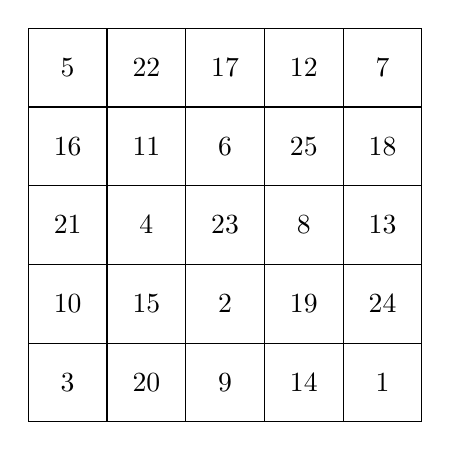
\begin{tikzpicture}
    \draw (0, 0)--(5, 0);
    \draw (0, 1)--(5, 1);
    \draw (0, 2)--(5, 2);
    \draw (0, 3)--(5, 3);
    \draw (0, 4)--(5, 4);
    \draw (0, 5)--(5, 5);
    \draw (0, 0)--(0, 5);
    \draw (1, 0)--(1, 5);
    \draw (2, 0)--(2, 5);
    \draw (3, 0)--(3, 5);
    \draw (4, 0)--(4, 5);
    \draw (5, 0)--(5, 5);
    \node at (0.5, 0.5) {3};
    \node at (4.5, 0.5) {1};
    \node at (2.5, 1.5) {2};
    \node at (1.5, 2.5) {4};
    \node at (0.5, 4.5) {5};
    \node at (2.5, 3.5) {6};
    \node at (4.5, 4.5) {7};
    \node at (3.5, 2.5) {8};
    \node at (2.5, 0.5) {9};
    \node at (0.5, 1.5) {10};
    \node at (1.5, 3.5) {11};
    \node at (3.5, 4.5) {12};
    \node at (4.5, 2.5) {13};
    \node at (3.5, 0.5) {14};
    \node at (1.5, 1.5) {15};
    \node at (0.5, 3.5) {16};
    \node at (2.5, 4.5) {17};
    \node at (4.5, 3.5) {18};
    \node at (3.5, 1.5) {19};
    \node at (1.5, 0.5) {20};
    \node at (0.5, 2.5) {21};
    \node at (1.5, 4.5) {22};
    \node at (2.5, 2.5) {23};
    \node at (4.5, 1.5) {24};
    \node at (3.5, 3.5) {25};
\end{tikzpicture}
\end{center}

\subsection*{ZAD. 12.}
\emph{Dany jest graf prosty $G$, w którym $n=|G|>3$ i dla dowolnych trzech wierzchołków $u,v,w\in G$ istnieją co najmniej dwie spośród trzech krawędzi $uv,vw,wu$. Wykaż, że w $G$ istnieje cykl Hamiltona.}
\medskip

\podz{sep}
\medskip

Weźmy dowolne $u,v\in G$ takie, że $uv\not\in G$. Wtedy dla dowolnego innego $w\in G$ musimy mieć $uw, vw\in G$. W takim razie dla dwóch dowolnych niepołączonych $u,v$ mamy
$$deg(u)+deg(v)=(n-2)+(n-2)=2n-4$$

co dla $n>3$ daje
$$deg(u)+deg(v)\geq n,$$
czyli z twierdzenia Orego wiemy, że w $G$ istnieje cykl Hamiltona.

\subsection*{ZAD. 15.}
\emph{Pokaż, że jeśli $G$ jest grafem prostym i dla każdej pary niesąsiednich wierzchołków $u,v$}
$$deg(u)+deg(v)\geq n(G)-1,$$
\emph{to w $G$ istnieje droga Hamiltona.}
\medskip

\podz{sep}
\medskip

Niech $G'$ będzie grafem $G$ z dodanym wierzchołkiem $w$ tak, że $(\forall\;v\in G)\;vw\in G'$. Teraz dla dowolnych niesąsiednich wierzchołków mamy
$$deg(u)+deg(v)\geq n.$$
Z twierdzenia Ore'a wiemy, że wtedy w $G'$ istnieje cykl Hamiltona. Niech teraz $C$ będzie tym cyklem i niech dla pewnych $v, u\in G$ $vw, uw\in C$. Wtedy jeśli usuniemy z $C$ te dwie krawędzie oraz wierzchołek $w$, to wrócimy do ścieżki zawartej w $G$, która przechodzi wszystkie wierzchołki.

% \subsection*{ZAD. 17.}
% \emph{Niech $G$ będzie grafem prostym. Pokaż, że $G$ zawiera drogę o długości równej co najmniej $2\cdot{e(G)\over |G|}$.}
% \medskip

% \podz{sep}
% \medskip

% Indukcja po ilości wierzchołków.
% \smallskip

% Dla $|G|=1$ jest to dość proste. Mamy $e(g)=0$, a więc $2\cdot{e(G)\over |G|}=2\cdot{0\over1}=0$.
% \smallskip

% Niech $|G|=n+1$ będzie grafem prostym, a $v\in G$ będzie wierzchołkiem o minimalnym stopniu $d=d(v)$. Wiemy, że $d\leq n-1$, bo $G$ jest prosty. Jeżeli teraz usuniemy wierzchołek $v$, to dostajemy $G'$ o $n$ wierzchołkach oraz $e(G)-d\geq e(G)-n+1$ krawędziach. W $G'$ możemy znaleźć ścieżkę o
% $$2\cdot {e(G')\over n}=2\cdot{e(G)-d\over n}\geq 2\cdot {e(G)-n+1\over n}\geq2\cdot{e(G)\over n+1}-\lfloor{2\cdot(n-1)\over n+1}\rfloor=2\cdot{e(G)\over n+1}-1$$
% czyli dodając nasz wierzchołek $v$ do tej ścieżki dostajemy ścieżkę długości $2\cdot{e(G)\over n+1}$. KONIEC.

\end{document}